\documentclass[]{article}
\usepackage[czech]{babel}
\usepackage[utf8]{inputenc}
\usepackage{float}
\usepackage{graphicx}


\begin{document}

\title{Kapitola 3: Notace BPMN}
\author{Bc. Štěpán Heller}
\date{\today}
\maketitle

\section{O BPMN}
BPMN neboli Business Process Modelling and Notation je soubor pravidel a grafických prvků, pomocí kterých mohou organizace modelovat svoje obchodní procesy. Jedná se pravděpodobně o světově nejpoužívanější standard pro modelování podnikových procesů. Jeho nespornou výhodou je, že narozdíl od hojně rozšířených vývojových diagramů, je BPMN standardizované, tudíž je možné modely vytvořené v BPMN automatizovat, je možné volně měnit nástroje, kterými jsou modely vytvářené a uživatelé tak nejsou závislí na jejich výrobcích. 

Za vznikem BPMN stála iniciativa BPMI (Business Process Management Initiative), jejíž primární motivací bylo vytvořit grafickou notaci, která bude srozumitelná všem účastníkům životního cyklu procesu (management, vývojáři, analytici) \cite{Vasicek2008}. Faktem je, že modely v BPMN v dnešní době slouží pro popis procesů na vysoké úrovni abstrakce, ale i pro popis těch nízkoúrovňových, které slouží jako podklad pro implementaci procesu v nějakém softwarovém nástroji.

Dalším cílem, se kterým bylo BPMN vytvořeno bylo ustanovit notaci, které umožní zobrazovat jednoduché i komplexní obchodní procesy \cite{Vasicek2008}, protože v té době obvyklé modelovací metody byly při vytváření rozsáhlých modelů velmi obtížně použitelné a vzniklé modely bylo složité udržovat.

O BPMN se dnes stará organizace Object Management Group (OMG). Za svojí popularitu vděčí BPMN, kromě výše zmíněných důvodů, zejména přístupnosti notace pro business uživatele, kteří jsou obeznámení s tradičními vývojovými diagramy, kterým se struktura diagramů i některé elementy v mnohém podobají \cite{Silver2011}. Rozdílem oproti vývojovým diagramům je ale již výše zmíněná standardizace použití jednotlivých e-mailů a tedy v tomto případě účelné omezení svobody uživatelů. Tento fakt umožňuje \textit{validovat} výsledné BPMN modely oproti specifikaci. Dalším rozdílem je možnost modelovat chování na základě výskytu nějaké definované události, což je situace, která se v reálném životě stává velmi často, ale ve vývojovém diagramu ji není možné vyjádřit. V neposlední řadě je v BPMN také možné modelovat komunikaci s entitami mimo organizaci nebo proces.

Jak tvrdí například \cite{Silver2011} v praxi vzniká velké množství \uv{špatného BPMN}, tedy modelů, které nejsou validní, kompletní nebo jednoznačné. Důvod je zřejmý – absence pevného teoretického základu, který by říkal více než k čemu který element z notace slouží a s kterým elementem je možné ho propojit. BPMN chybí \textit{metodologie}, která by přesně popisovala jak modely vytvářet a jak zaručit jejich konzistenci, jednoznačnost a kompletnost. V praxi tedy vidíme vznik metodologií, které nejsou součástí standardu BPMN, ale jsou adoptovány ve firmách právě z důvodu požadavků na výše zmíněné vlastnosti a rovněž pro zajištění kontinuity. Jednou z velmi rozšířených je metoda popsaná v publikaci \textit{BPMN Method and Style} vyvinutá Brucem Silverem, který se rovněž podílí na vývoji standardu BPMN. Cílem metody je jejím dodržováním vyvářet modely, které jsou

\begin{itemize}
\item korektní,
\item jednoznačné,
\item kompletní,
\item konzistentní.
\end{itemize}

\begin{quote}
\uv{Špatné BPMN} je dnes normou spíše než výjimečností. \cite{Silver2011}
\footnote{Bad BPMN is the norm rather than the exception. \cite{Silver2011}}
\end{quote}

\subsection{Verze 1.2 vs 2.0}
BPMN je v současnosti ve verzi 2.0, nicméně v praxi je stále hojně využívána i verze 1.2. Klíčovým rozdílem je standardizace převodu BPMN konstruktů do jazyka XML, což by umožnilo z grafického vyjádření modelu v notaci BPMN vygenerovat metamodel v jazyce XML, který by bylo možné automatizovat pomocí softwarových nástrojů. Taková řešení sice již existovala i u starších verzí BPMN, ale byla vždy závislá na interpretaci výrobce konkrétního BPMS řešení a tudíž jen obtížně přenositelná. Standard BPMN 2.0 by měl toto změnit. Co se týče grafických elementů, tak do verze 2.0 jich oproti 1.2 přibylo jen velmi málo a většina business uživatelů tak pravděpodobně ani rozdíl nepostřehne.

\section{Základní koncepty notace BPMN}
Dříve než přikročíme k popisu základních elementů notace BPMN

\subsection{BPMN diagram}
Diagram v BPMN není pouze grafickým vyjádřením podnikového procesu, ale zároveň vstupním budem pro \textit{sémantický model} v jazyce XML, který je (pokud to modelovací software umožňuje) vytvářen zároveň s grafickým diagramem aniž by do toho uživatel musel jakkoli zasahovat. Jak píše \cite{Silver2011} BPMN dovoluje existenci sémantického modelu bez jeho grafického vyjádření, ale ne naopak – sémantický model tedy musí vždy existovat.

Procesní model v BPMN neříká nic o tom, jak jsou jeho jednotlivé aktivity prováděny nebo proč jsou prováděny. Definuje pouze následující:

\begin{itemize}
\item \textit{pořadí} aktivit,
\item \textit{kdy} se aktivity provádějí,
\item za jakých \textit{podmínek} se aktivity provádějí.
\end{itemize}

\subsection{Aktivita v BPMN}
\cite{Silver2011} definuje \textit{aktivitu} v BPMN jako \textit{akci}, jednotku provedené práce. Aktivita je akce prováděná v rámci organizace opakovaně a je neměnná, neboli je vždy prováděna stejným způsobem a má jasně vymezený začátek a konec. Aktivita je v rámci modelu dále nedělitelná, tj. není možné ji rozložit na subaktivity.

\subsection{Proces v BPMN}
Samotný pojem \textit{proces} lze v BPMN jednoduše popsat jako posloupností aktivit z počátečního stavu do konečného stavu \cite{Silver2011}. \textit{Procesní model} je pak mapou všech možných cest – posloupností aktivit – z počátečního stavu do některého z konečných stavů. Podobně jako aktivita i proces je prováděn opakovaně a každá jeho instance musí být prováděna dle některé z cest definovaných v procesním modelu.

Dle \cite{Silver2013} má proces v BPMN 4 důležité aspekty:

\begin{itemize}
\item \textbf{Orchestrace} – jako orchestraci označujeme fakt, že procesy v BPMN se skládají z aktivit, které jsou vždy prováděny v určitém pořadí tak, jak je definováno v procesním modelu. Tyto aktivity jsou prováděny opakovaně a průběh jejich vykonávání má jasně definovaný začátek a konec. Procesní model navíc obsahuje všechny signifikatní možnosti, jak proces může proběhnout, ne jen jednu nejčastější nebo ad-hoc případy provádění.
\item \textbf{Participant} – samotný proces v BPMN je vnímán jako samostatná entita a je účastníkem \textit{spolupráce (collaboration)} s jinými entitami. Každý participant je unikátně propojen s jedním procesem.
\item \textbf{Množina vykonavatelů} – každá aktivita v BPMN má vykonavatele ač není v diagramu znázorněn. Pokud je aktivita součástí orchestrace popsané výše, je pak součástí procesu a to samé platí i pro jejího vykonavatele.
\item \textbf{Nezávislý actor} – BPMN používá z hlediska reálného života poměrně neobvyklou sémantiku, kdy u aktivity je tím, kdo požaduje její vykonání \textit{samotný proces} (jeho instance) a aktivitu provádí její vykonavatel (například zaměstnanec).
\end{itemize}

\subsection{Procesní logika}
\textit{Procesní logika} definuje všechny signifikatní možnosti, jak může proces probíhat (sekvence aktivit) od začátku do konce. Každý procesní model by měl obsahovat kompletní procesní logiku, pokud pro vypuštění některých možných cest neexistuje vážný důvod. Častým problémem modelů, které \cite{Silver2011} označuje jako \uv{špatné BPMN} je popis pouze jedné cesty (obvykle té \uv{šťastné}, tzv. \textit{happy flow}) a ignorování případů, které z nějakého důvodu probíhají odlišně.

\section{Základní elementy notace BPMN}

Standard BPMN ve verzi 2.0 obsahuje již více než 100 symbolů. Popis všech je mimo rozsah této práce. Nicméně v této sekci budou popsány všechny elementy, které populární publikace \cite{Silver2011} označuje jako \textit{Level 1} a několik vybraných elementů z množiny, které stejný autor označuje jako \textit{Level 2}, které se nám budou hodit později v dalších částech práce.

Symbolika použitá v BPMN je odvozená od klasické a hojně rozšířené flowchartovací techniky, která je intuitivní na pochopení i pro pozorovatele, který není obeznámen s problematikou modelování podnikových procesů.

Jak uvádí \cite{Silver2011} a \cite{Vasicek2008} pro základní práci obvykle stačí pouze základní druhy elementů, které jsou:

\begin{itemize}
\item Počáteční událost (Start event)
\item Konečná událost (End event)
\item Aktivita (Activity)
\item Sekvenční tok (Sequence flow)
\item Tok zpráv (Message flow)
\item Brána (Gateway)
\item Bazén (Pool)
\item Plavecká dráha (Swimming lane)
\item Datový objekt (Data object)
\item Datové úložiště (Data store)
\item Datová asociace (Data association)
\end{itemize}

Pro potřeby této práce si ještě popíšeme následující elementy:

\begin{itemize}
\item Signál (Signal)
\item Průběžná událost (Intermediate event)
\end{itemize}

\subsection{Aktivita}
\textit{Aktivita} je v procesu graficky znázorněna obdélníkem se zaoblenými rohy. Jak již bylo popsáno výše, reprezentuje jednotku provedené práce. Jako jediný BPMN element má \textit{vykonavatele} \cite{Silver2011}. 

\begin{figure}[H]\centering

\includegraphics{obrazky/activity}
\caption{Element Aktivita}
\label{fig:aktivita}
\end{figure}

Každá aktivita je buď \textit{task (Task)} nebo \textit{subproces (Subprocess)}. Task je atomický typ aktivity, tedy v modelu jej není možné rozdělit na další aktivity, ze kterých se skládá narozdíl od subprocesu, který je definované má a v modelu jsou znázorněné jako samostatný proces s počátečním i koncovým stavem. V závislosti na preferenci uživatele může být subproces zobrazen v rodičovském procesu jako jedna \uv{sbalená} aktivita nebo jsou přímo v rodičovském procesu vidět všechny aktivity, které subproces obsahuje. Subproces musí vždy začínat \textit{počáteční událostí typu None}. Task se dělí na 8 podtypů, jejichž definice je k dohledání ve specifikaci \cite{Omg2011}. V rámci této práce budeme používat pouze abstraktní task.

\subsection{Brána}
V případě, že je potřeba rozštěpit sekvenční tok, obvykle na základě nějaké podmínky, je tu element \textit{brána}. Bez použití brány není možné sekvenční tok rozdělit, narozdíl například od vývojových diagramů. Brána je v BPMN diagramu zobrazena použitím kosočtverce nepovinně se symbolem uvnitř. Existuje několik typů bran:

\begin{itemize}
\item Exkluzivní (XOR)
\item Paralelní (AND)
\item Inkluzivní (OR)
\item Komplexní
\item Event-based
\end{itemize}

\begin{figure}[H]\centering
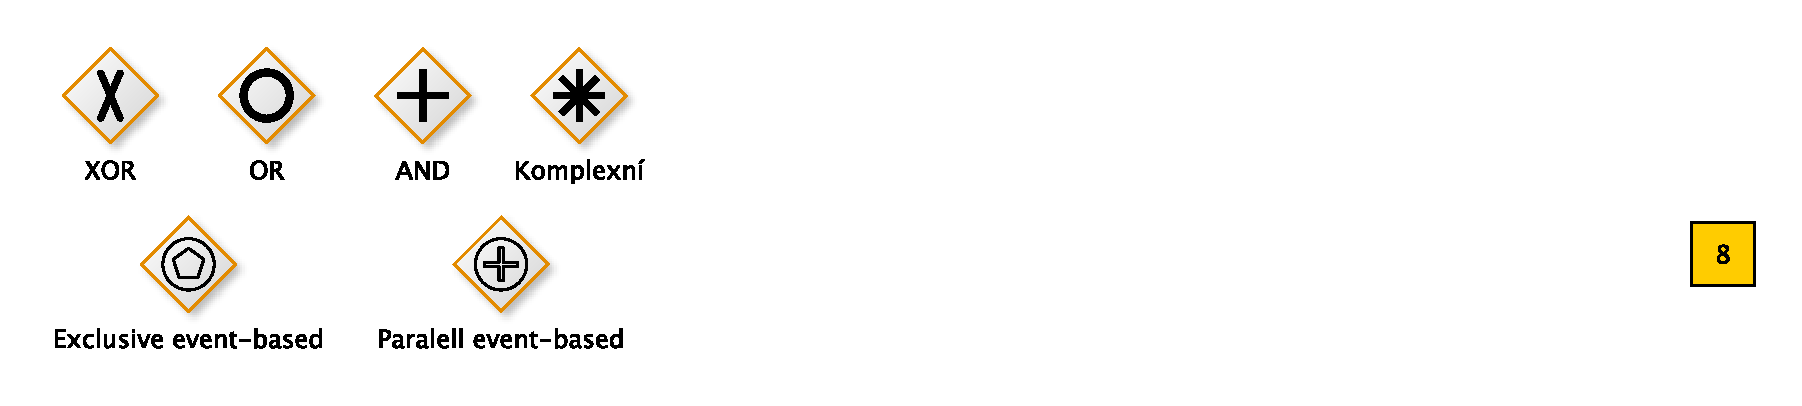
\includegraphics{obrazky/gateway-types}
\caption{Různé druhy elementu Brána}
\label{fig:brany}
\end{figure}

\subsubsection{Ekluzivní brána (XOR)}
Fungování exkluzivní brány je poměrně přímočaré. Jak už jméno naznačuje, tato brána umožní pokračovat pouze jednomu sekvenčnímu toku na svém výstupu. Rozhodnutí v bráně by měla předcházet aktivita, která provede samotné rozhodnutí a brána by pak již jen \uv{ověřila} výsledek tohoto rozhodnutí a příslušně němu vybrala na výstupu sekvenční tok.

\subsubsection{Paralelní brána (AND)}
I v tomto případě je chování brány předvídatelné. Paralelní brána rozdělí vstupní sekvenční tok na více výstupních toků, po kterých proces pokračuje bez jakékoli podmínky. Paralelní bránu lze využít i v případě, kdy potřebujeme různé sekvenční toky opět spojit a je nutné zajistit jejich synchronizaci, tj. vyčkat na všechny příchozí sekvenční toky a teprve v momentě, kdy dorazí všechny, pokračovat v procesu.

\subsubsection{Inkluzivní brána (OR)}
Inkluzivní brána narozdíl od exkluzivní varianty umožňuje na základě splněné podmínky na výstupu $1...n$ aktivních sekvenčních toků.

\subsubsection{Komplexní brána}
Komplexní brána se využívá pouze v případě, kdy není možné rozdělení sekvenčního toku modelovat použitím jiného typu brány. Lze ji vidět použitou v momentech, kdy rozdělení sekvenčního toku předchází nějaké velmi komplexní rozhodnutí. Podmínky, za kterých je použit určitý výstupní sekvenční tok jsou specifikovány textovým popisem na jednotlivých větvích sekvenčního toku.

\subsubsection{Event-based brána}
Event-based brána se používá v případě, kdy o výběru výstupního sekvenčního toku \uv{rozhodne} situace, kdy nastala nějaká událost (například obdržení zprávy).

\subsection{Počáteční a konečná událost}
Každý proces v BPMN by měl začínat nějakým typem počáteční události a končit v některém typu konečné události. Obě tyto události jsou zobrazeny pomocí kruhu, který může obsahovat symbol určující, o jaký typ události se jedná. Proces může mít více počátečních událostí (speciální typy procesů naopak žádnou) a víc konečných událostí.

Symbol uvnitř kruhu označuje, o jaký typ počáteční nebo konečné události se jedné. V případě té počáteční symbol označuje jev, který proces spouští (například zpráva nebo signál). Počáteční událost může mít následující typy:

\begin{itemize}
\item Prázdný (None)
\item Zpráva (Message)
\item Časovač (Timer)
\item Multiple a Multiple-Parallel
\end{itemize}

\begin{figure}[H]\centering

\includegraphics{obrazky/start-events}
\caption{Různé druhy Počátečních událostí}
\label{fig:pocatecni_udalosti}
\end{figure}

BPMN 2.0 define 9 typů konečných událostí, ale v praxi se používají zejména tyto 4: \cite{Silver2011}

\begin{itemize}
\item Prázdný (None)
\item Zpráva (Message)
\item Terminate
\item Multiple
\end{itemize}

\begin{figure}[H]\centering

\includegraphics{obrazky/end-events}
\caption{Různé druhy Konečných událostí}
\label{fig:konecne_udalosti}
\end{figure}

\subsubsection{Prázdná počáteční událost}
Prázdná počáteční událost se používá v případech, kdy proces není spouštěn žádným jevem nebo tento jev není specifikován. Často se tento typ počáteční události využívá v případě, kdy je proces spouštěn manuálně vykonovatelem určitého tasku.

\subsubsection{Počáteční událost typu Zpráva}
Proces jehož počáteční událost je typu zpráva se spouští okamžikem přijetí nějaké specifické zprávy, kterou zašle jiný proces.

\subsubsection{Počáteční událost typu Časovač}
Pokud je projekt spouštěn pravidelně v určitý čas dle nějakého plánu, používá se počáteční událost typu Časovač. Štítek (Label) počáteční události tohoto typu by měl vyjadřovat frekvenci s jakou je proces spouštěn (např. \textit{denně}, \textit{kvartálně}).

\subsubsection{Prázdná konečná událost}
Pokud proces končí v prázdné konečné události znamená to zjednodušeně řečeno, že o svém konci proces nedá veřejně vědět, jelikož není vyslán žádný signál nebo zpráva.

\subsubsection{Konečná událost typu Zpráva}
Konečná událost typu zpráva je reprezentována kruhem s černou obálkou uvnitř. Tento typ konečné události vyjadřuje, že proces při svém ukončení vyšle zprávu nějakému jinému procesu.

\subsubsection{Konečná událost typu Terminate}
Konečná událost typu Terminate se používá v případě speciálních událostí, kdy je potřeba v případě dosažení tohoto konečného stavu ukončit i všechny aktivní paralelní sekvenční toky, podprocesy atd.

\subsection{Sekvenční tok}
Sekvenční tok je v diagramu zobrazen pomocí nepřerušované šipky, která je vždy připojena z obou stran k jiným BPMN elementům v diagramu. Jeho úkolem je určovat pořadí provádení aktivit v procesu. Sekvenční tok dle specifikace může propojovat pouze aktivity, brány a události. Jinými slovy sekvenční tok reprezentuje \textit{orchestraci}. \cite{Silver2011}

U sekvenčních toků je velmi důležité mít na paměti pravidlo, že žádný sekvenční tok nesmí nikdy překročit hranice subprocesu nebo bazénu, neboť toto chování specifikace BPMN zapovídá.

\subsection{Tok zpráv}
Narozdíl od sekvenčního toku je tok zpráv v diagramu zobrazen šipkou s přerušovanou čárou. Vyjadřuje zaslání zprávy od odesílatele k příjemci, kterým je nějaká externí entita (black-box bazén nebo aktivita, zpráva nebo událost uvnitř jiného procesu). Je důležité si uvědomit, že tok zpráv neindikuje vždy jistotu, že komunikace opravdu proběhne. Někdy se jedná jen o vyjádření, že je v tomto momentě možné odeslat nebo přijmout zprávu.

\subsection{Bazén a plavecké dráhy}
Jasně ohraničený obdélník orientovaný vertikálně či horizontálně ohraničuje \textit{bazén}. Bazén slouží k vymezení hranic mezi procesem a externími entitami. Bazén obsahuje BPMN elementy procesu nebo se jedná o tzv.\textit{ black-box bazén}. Ten se používá v případě, že chceme modelovat komunikaci s externí entitou, ale nechceme zobrazovat jak vnitřní entita funguje.

\begin{figure}[H]\centering
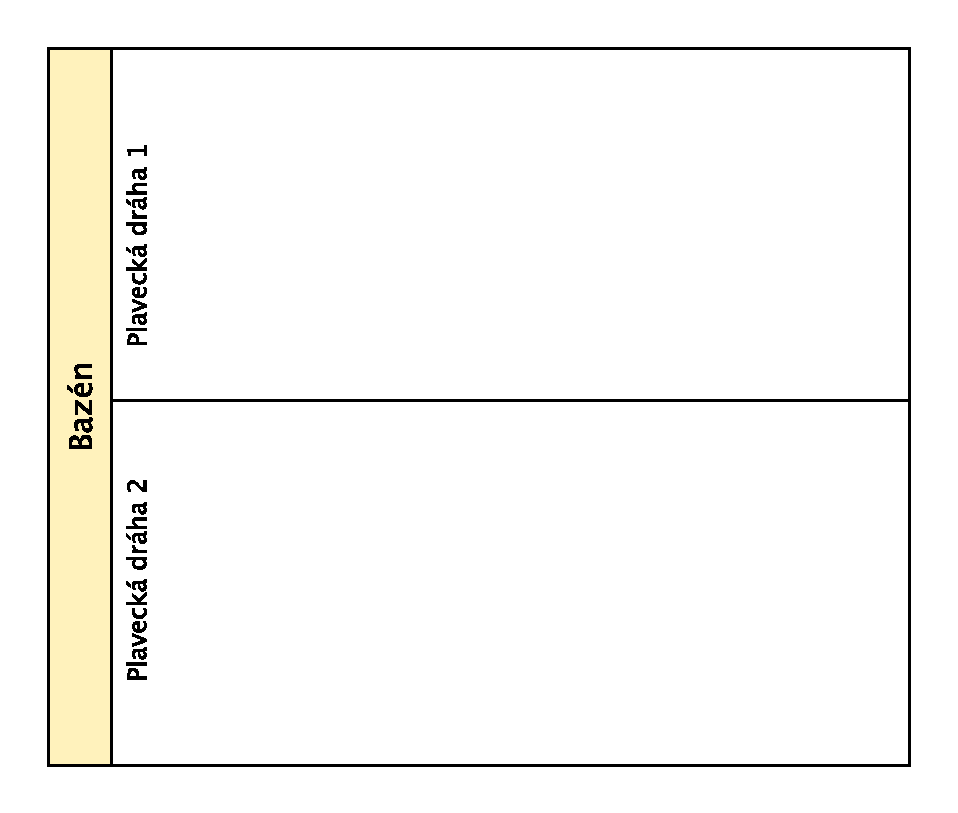
\includegraphics[scale=0.7]{obrazky/pool-swimming_lane}
\caption{Element Bazén s Plaveckými drahami}
\label{fig:bazen}
\end{figure}

\textit{Plaveckou dráhu} je možné použít v bazénu i mimo něj. Používá se většinou k zachycení rozdělení odpovědností za danou aktivitu v rámci organizace, nicméně specifikace BPMN 2.0 dovoluje prakticky neomezené použití plaveckých drah k jakémukoliv typu kategorizace. \cite{Silver2011}

Grafická reprezentace se podobá bazénu, nicméně rozdíl je ve štítku vlevo, který u plavecké dráhy není ohraničen a oddělen od zbytku elementu. V jednom bazénu bývá typicky více plaveckých drah, nicméně plavecku dráhu je možné zobrazit i vně bazénu.

\subsection{Datový objekt, úložiště, asociace}
Reprezentace dat a práce s nimi došla v BPMN 2.0 výrazné změny, kdy \textit{datový objekt} je v nové verzi plnohodnotným BPMN elementem a zároveň byl přidán nový objekt \textit{datové úložiště}.

Datový objekt je graficky reprezentován elementem, který připomíná list papíru s ohnutým rohem a jedná se spíše o programátorský konstrukt, jak uvádí \cite{Silver2011}. Reprezentuje lokální proměnnou, data, která existují dočasně v rámci instance procesu.

Datové úložiště oproti tomu reprezentuje data, která jsou dostupná trvale, například v nějaké databázi nebo na jiném místě. Data je možné z procesu číst či měnit. Datové úložiště je symbolem válce se třemi čárkami ve vrchní části.

S ostatními elementy v procesu jsou výše popsané datové objekty spojené prostřednictvím datových asociací, které jsou znázorněny tečkovanými šipkami s nevyplněným V na vrcholu nebo bez něj.

\begin{figure}[H]\centering

\includegraphics[scale=0.7]{obrazky/data-object-store}
\caption{Element Datový objekt a Datové úložiště}
\label{fig:datove_objekty}
\end{figure}

\section{Základní pravidla modelování v BPMN}
Specifikace BPMN předepisuje poměrně málo pravidel, jak modely vytvářet ve smyslu jak elementy používat a jak ne. Je tedy běžné, že pravidla vznikají přirozeně uvnitř organizací, kde chtějí sjednotit styl, podle kterého modely vznikají, aby byly modely vzniklé uvnitř organizace navzájem kompatibilní.\cite{Silver2011} uvádí, že BPMN má 3 zdroje, ze kterých lze pravidla vyčíst a těmi jsou:

\begin{itemize}
\item oficiální specifikace,
\item BPMN metamodel,
\item XML schéma příslušné metamodelu.
\end{itemize}

V této sekci najdeme přehled nejdůležitějších oficiálních pravidel dle specifikace BPMN, které by měl dodržovat každý model vzniklý v BPMN a měl by být proti nim validován.

\begin{enumerate}
\item Sekvenční tok nesmí překročit hranice bazénu.
\item Sekvenční tok nesmí překročit hranice podprocesu.
\item Tok zpráv nesmí spojovat elementy uvnitř stejného bazénu.
\item Sekvenční tok může spojovat mezi sebou pouze aktivity, brány, události a oba konce sekvenčního toku musí být k některému z těchto elementů připojené.
\item Tok zpráv může spojovat pouze aktivity, události (typu Zpráva nebo Multiple) nebo hranice black-box bazénu a oba konce musí být k některému z těchto elementů připojené.
\end{enumerate}

\section{Možnosti automatizace BPMN modelů}
Čím dál častěji jsou v dnešní době BPMN modely vytvářeny ne pouze za účelem jejich zdokumentování, ale stále více také za účelem jejich budoucí automatizace. \cite{Leymann2009} Myšlenka na automatizaci procesních modelů však existovala již na samotném začátku, kdy BPMN vzniklo jako grafická vrstva v rámci systému vyvíjeného konsorciem BPMI.org. \cite{Silver2011} Vznikl tak jazyk BPML, který měl být nezávislým standardem pro automatizaci procesů a popis procesu v jazyce BPML by nebyl \uv{programován}, ale generován automaticky z diagramu v notaci BPMN. BPML se ale nikdy neuchytil, společnosti IBM a Microsoft vyvinuly vlastní jazyk BPEL, který staví na standardu pro webové služby WSDL, a tento jazyk rychle na trhu BPML jasně předčil.

Kromě některých proprietárních řešení, které zde popsány nebudou, stojí za popsání dvě řešení automatizace BPMN, kterými jsou BPMN 2.0 a BPEL.

\subsection{BPMN 2.0}
BPMN 2.0 se od předchozí verze s označením BPMN 1.2 ve skutečnosti co se nových elementů a jejich vzhledu liší jen velmi málo. Hlavní změny se odehrály tak říkajíc pod povrchem na \textit{metamodelu} a na jeho reprezentaci v jazyce XML. Hlavním cílem těchto změn bylo vytvořit standardizovaný XML formát popisující model procesu, který bude sloužit vzájemné kompatibilitě modelů mezi různými BPMN nástroji a zároveň umožní modely automatizovat \cite{Silver2011}. 

BPMN 2.0 tak standardizuje reprezentaci dat v procesu, zpráv, služeb, přidělení tasků apod. v XML, které je vytvářeno spolu s každým diagramem. Jak uvádí \cite{Silver2011}, pro každý BPMN element je nutno specifikovat parametry jako:

\begin{itemize}
\item Proměnné procesu
\item Data na vstupu i výstupu tasku a jejich vazby na proměnné
\item Zprávy
\item Definice událostí
\item Podmíněné výrazy
\end{itemize}

Jak poznemenává \cite{Siver2011}, BPMN 2.0 narozdíl od BPEL popsaného níže není jazykem pro popis automatizace procesů a tedy není možné v BPMN 2.0 procesy přímo spouštět. Každý softwarový nástroj bude muset implementovat vlastní exekuční prostředí pro BPMN 2.0 XML metamodel. V současnosti však není adopce této části BPMN 2.0 u výrobců softwarových nástrojů příliš markantní. \cite{Silver20112}

\subsection{BPEL}
BPEL neboli Business Process Execution Language (přesněji WS-BPEL Web Service Business Process Execution Language) je jazyk pro popis automatizace procesů. Je založený na XML, ve kterém popisuje veškeré detaily o procesu a jeho elementech. Proces popsaný v BPEL je možné přímo spouštět v některém z dostupných BPEL exekučních prostředí.

Jazyk BPEL nemá žádnou oficiální grafickou reprezentaci, ale jelikož většina business uživatelů chce procesní modely vytvářet v uživatelsky příjemném grafickém editoru a ne pomocí programovacího jazyka, používá každý z BPEL nástrojů nějakou grafickou notaci, kterou následně převádí do BPEL. Tato notace může být proprietární (vyvinutá výrobcem nástroje), častěji se však využívá notace BPMN, se kterou jsou uživatelé dobře obeznámeni.

Jak již bylo uvedeno výše, oficiální název pro BPEL je WS-BPEL, kde první dvě písmena znamenají Web Service neboli \textit{webová služba}. Celý jazyk BPEL je založen na WSDL neboli Web Service Description Language. Jednou z jeho základních funkcí tak je orchestrace webových služeb. Úkolem BPEL je integrace funkcionalit, které postkytují webové služby pro implementaci v konkrétním podnikovém procesu.

Proces v BPEL je popsán pomocí XML dokumentu, který popisuje veškeré elementy a umožňuje popsat i vztahy mezi nimi a také s webovými službami. Tento XML dokument je pak spustitelný pomocí exekučního prostředí.

Jako již bylo zmíněno výše, BPMN je velmi často využíváno pro modelování procesu na grafické úrovni a takový model je pak převeden do BPEL. Že je to velmi běžná praxe napovídá i samotná specifikace jazyka BPMN, která přímo obsahuje informace o tom, jak BPMN do BPEL převádět. \cite{Cerny2010}


\nocite{*}
\bibliographystyle{plain}
\bibliography{Bibliography}

\end{document}